%!TEX root = ../ENTRUST_TR.tex
This section will explain how we achieved our goal.

\subsection{Managed System}
Details about managed system

\subsection{Managing System}
In this section, we briefly describe the managing system automata. 

\subsubsection{Monitor}
Monitor automaton receives the sensors rates from probes. After that, the monitor automaton checks that whether received sensor rates are equal to previously measured sensor rates. If both rates are equal, then there is no need to analyze because an analysis already have been applied to these sensor rates. If sensor rates are different then analysis is required and the monitor automaton will invoke the analyze automaton by sending an \textit{start\_analysis!} signal as shown in Fig.~\ref{fig:monitor-automaton}. 

\begin{figure}[t]
	\centering
	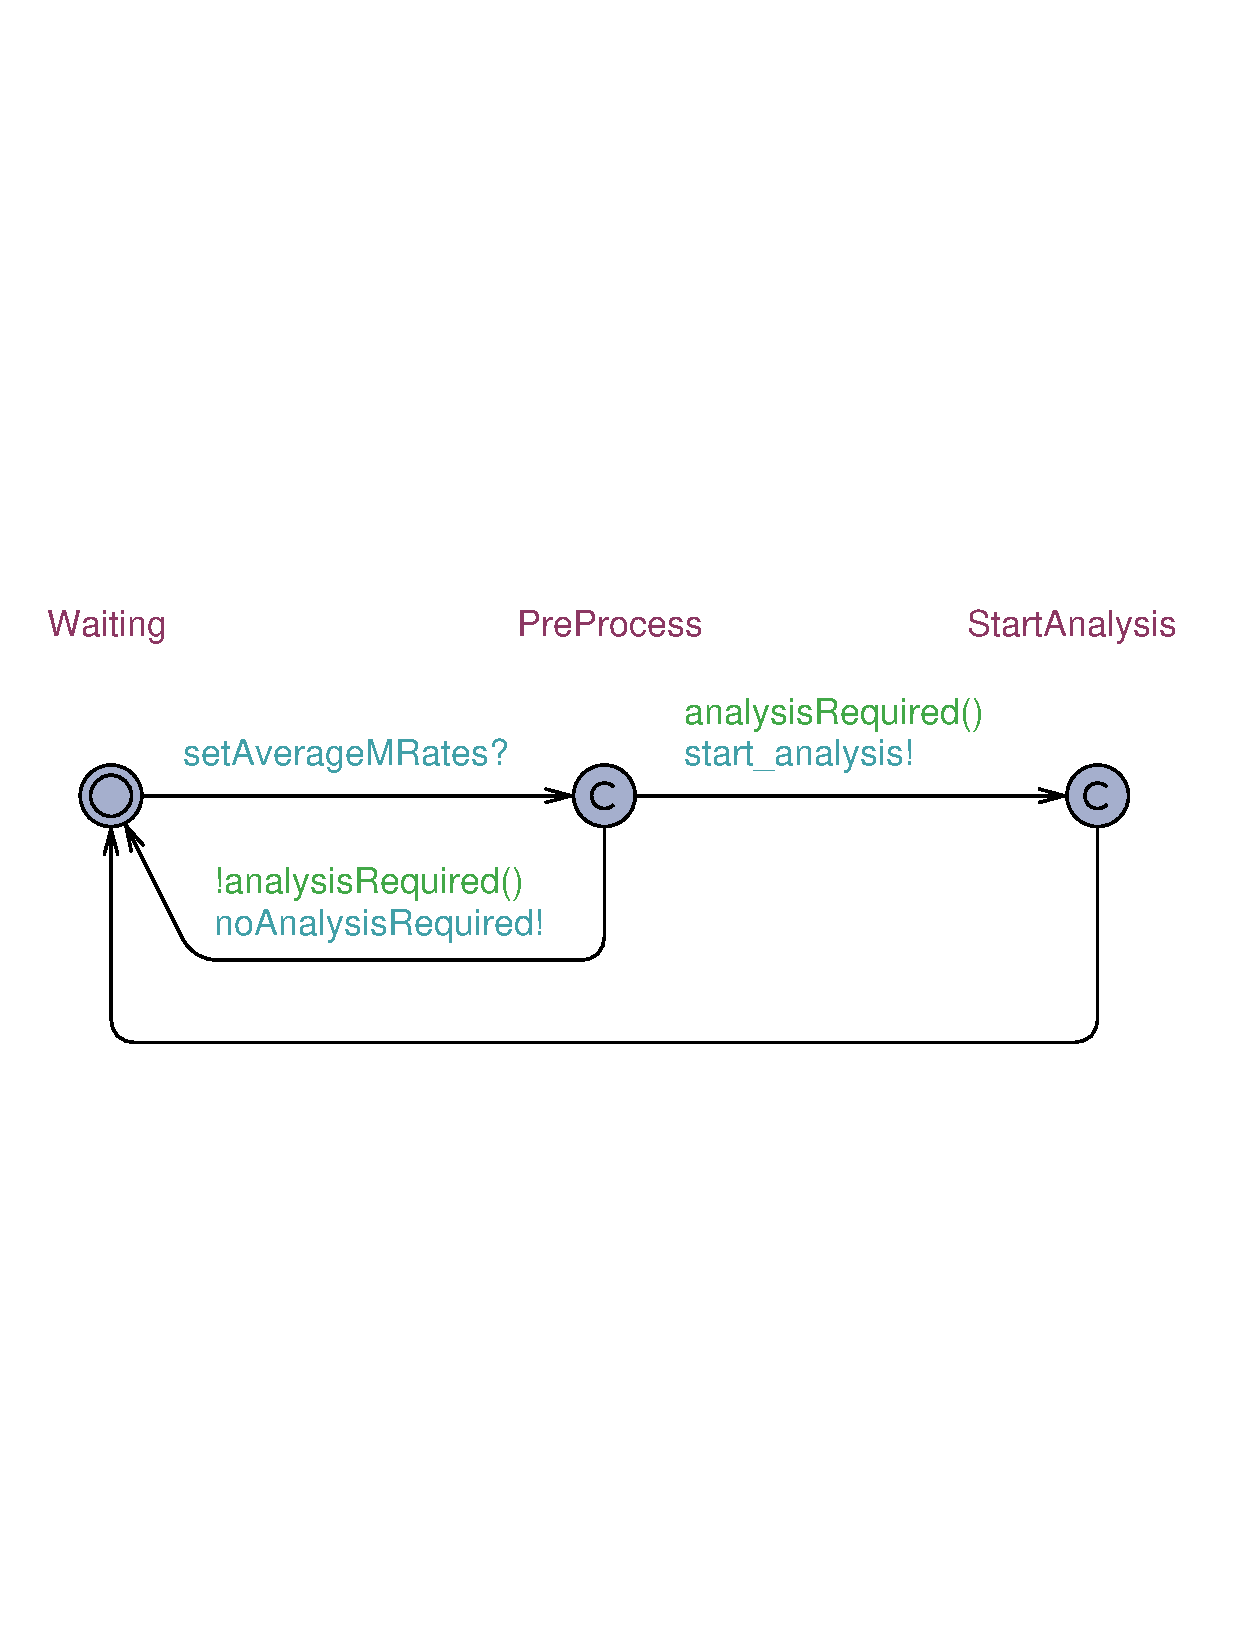
\includegraphics[width=0.5\textwidth]{figures/Monitor}
	\caption{Monitor automaton of UUV}\label{fig:monitor-automaton}
	
	\vspace*{-2mm}
\end{figure}

\subsubsection{Analyze}
Analyze automaton takes the current measured rates of sensors and try to find the best configuration which fulfills the requirement R1, R2 and R3. Fig.~\ref{fig:analysis-automaton} shows the analyze automaton of feedback loop. The analyze automaton starts the analysis when received the signal \textit{start\_analysis?} from monitor automaton. After receiving the signal from monitor automaton, the analyze automaton sends the sensor rates to RQV by sending the signal ~\textit{calcProbability}.
When the RQV receive the signal it creates a set of possible configurations and send back to the analyze automaton through ~\textit{recvProbability?} channel. After that the analyze automaton analyzes the set of configurations and try to find a best configuration which holds the R1, R2 and R3. Once the best configuration is found, the analyze automaton compares the current configuration of UUV to the best configuration. If both configurations are equal, then there is no need to plan anything. If the best configuration is not equal to the current configuration of UUV, the analyze automaton recognize that this is the time to do an adaptation, and send the signal ~\textit{planning!} to invoke the planner. Fig.~\ref{fig:analysis-automaton} shows the analyze automaton of the UUV.


\begin{figure}[t]
	\centering
	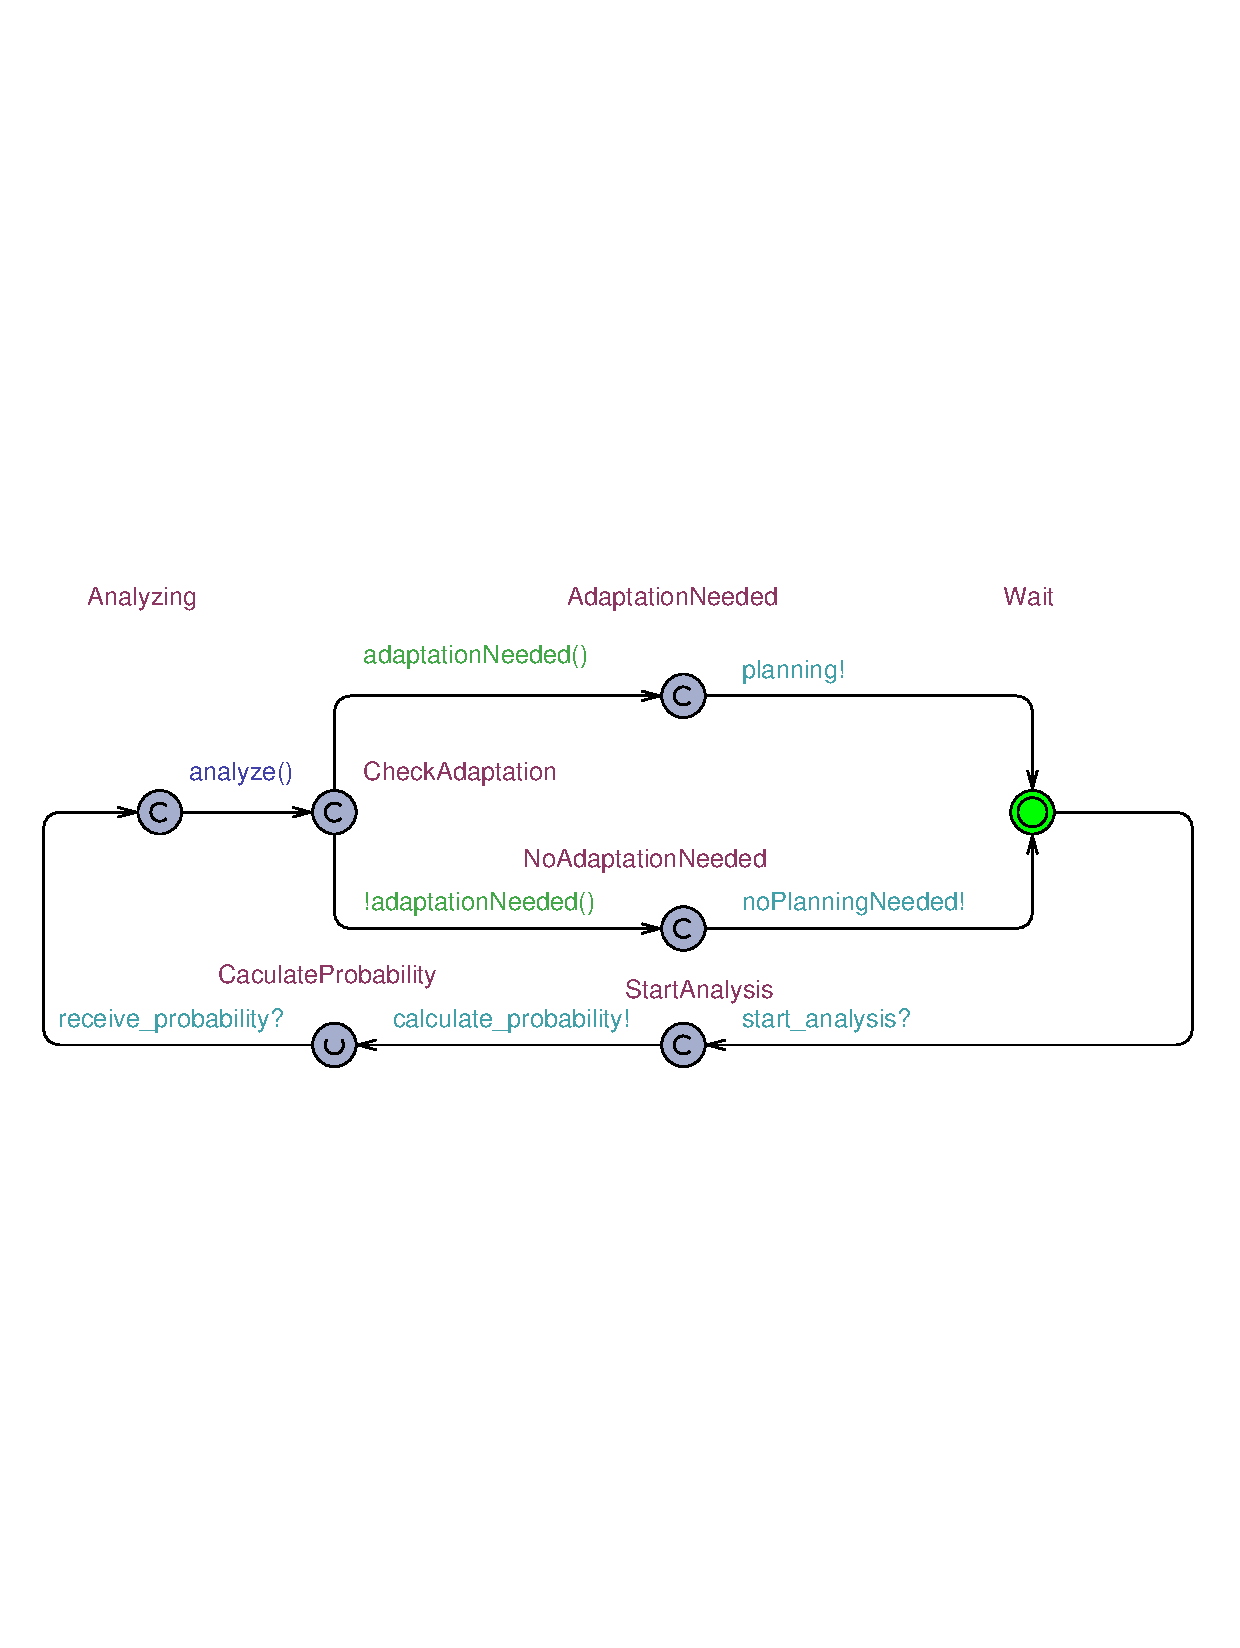
\includegraphics[width=0.7\textwidth]{figures/Analyzer}
	\caption{Analyze automaton of UUV}\label{fig:analysis-automaton}
	
	\vspace*{-2mm}
\end{figure}


\subsubsection{Plan}
Plan automaton creates the plans for adaptation. The plan automaton starts the planning when the signal ~\textit{planning?} is received. The plan automaton starts first with creating the plan steps for sensor configuration, i.e., whether a sensor should be turned on or off. To do that, the plan automaton checks the current sensor configuration with the best configuration for each sensor to determine whether there is a need to turn on the sensor or off. If the sensor configuration is same as in the best configuration, then there is no need to create a plan step. Otherwise, if sensor configurations are not matched then the plan automaton creates the plan step, according to the best configuration. When all sensors are checked, then the plan automaton checks the current speed of the UUV with the UUV speed in best configuration. Similarly, if the current UUV speed doesn't match with the speed in best configuration, the plan automaton creates a new plan step to change the speed of UUV, otherwise the plan automaton continues. After checking the UUV speed, the plan automaton invokes the execute automaton by sending the ~\textit{execute!} signal. Fig.~\ref{fig:plan-automaton} shows the plan automaton of the UUV.
\begin{figure}[t]
	\centering
	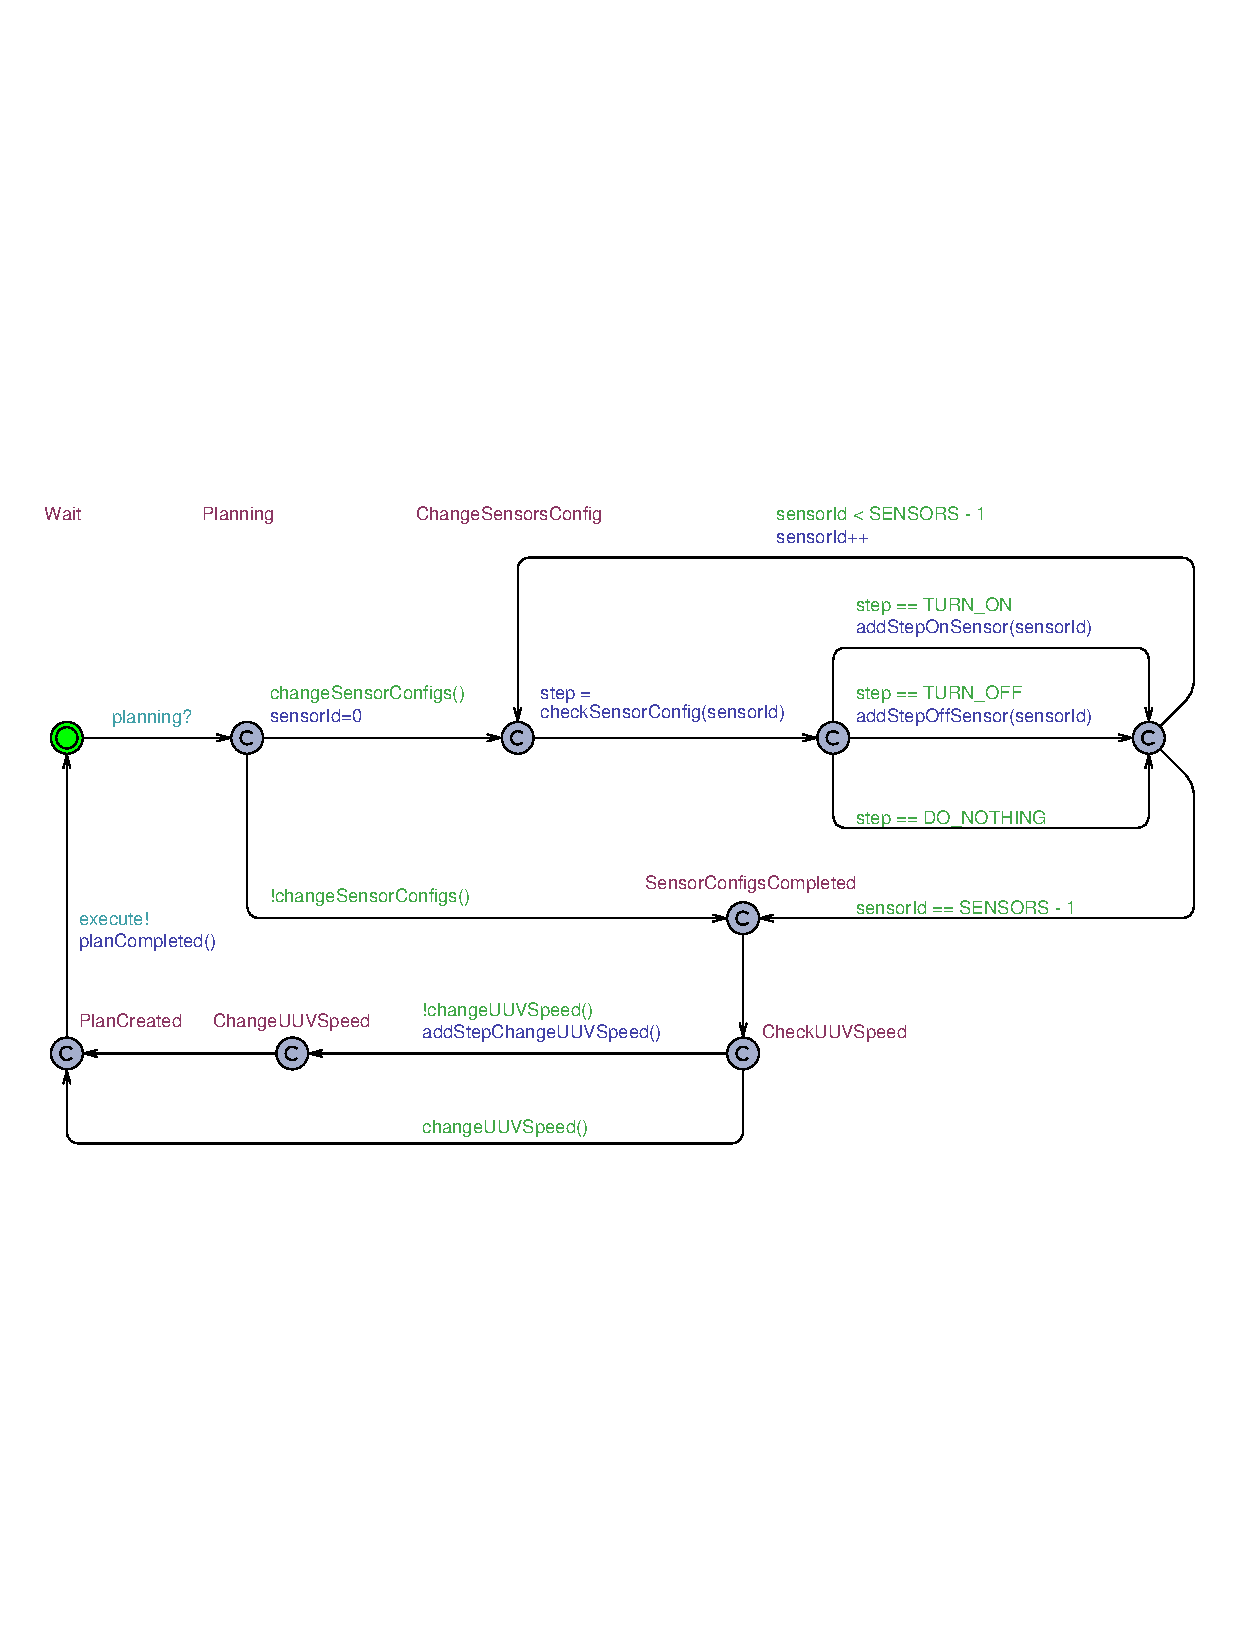
\includegraphics[width=1\textwidth]{figures/Planner}
	\caption{Plan automaton}\label{fig:plan-automaton}
	
	\vspace*{-2mm}
\end{figure}


\subsubsection{Execute}
The execute automaton starts by the signal ~\textit{execute?} sent from the plan automaton. After receiving the signal the execute automaton goes through all the plan steps one by one and execute them. The plan automaton is presented in the Fig.~\ref{fig:execute-automaton}.

\begin{figure}[t]
	\centering
	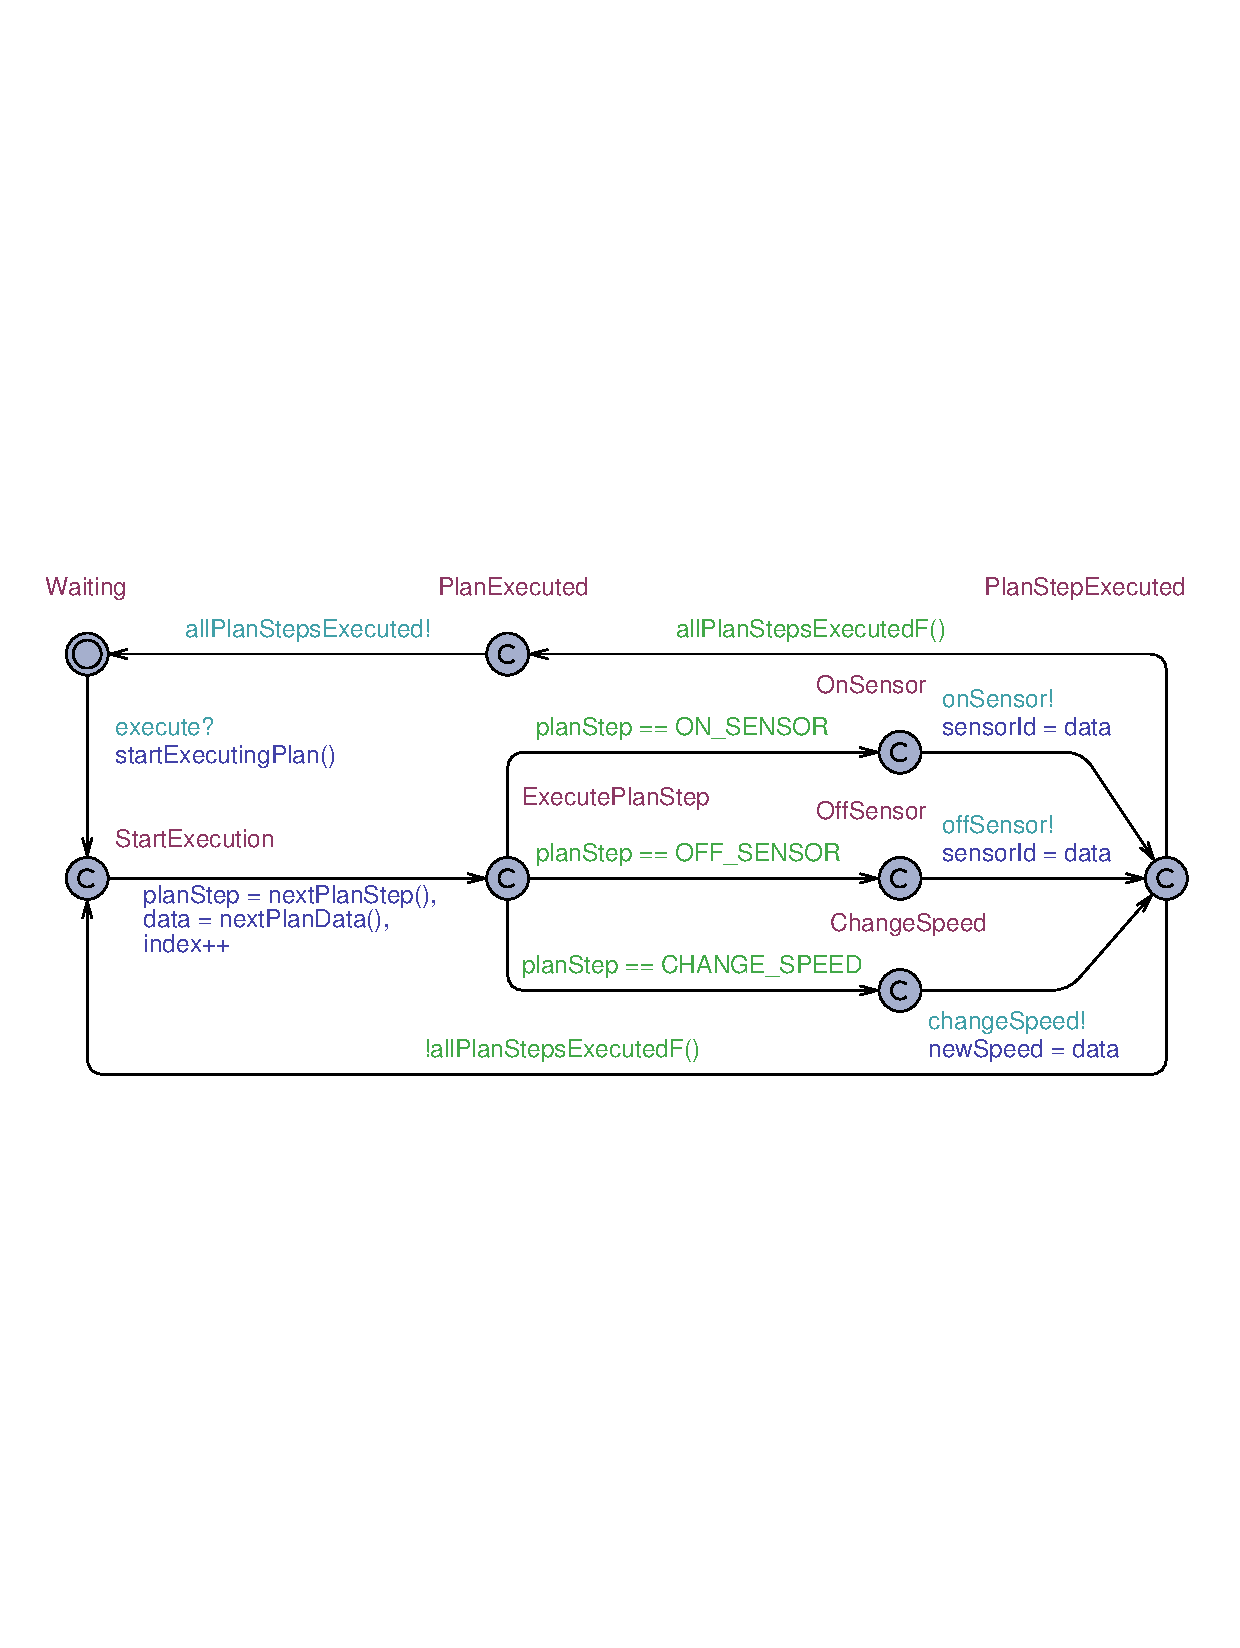
\includegraphics[width=1\textwidth]{figures/Executor}
	\caption{Execute automaton}\label{fig:execute-automaton}
	
	\vspace*{-2mm}
\end{figure}


\subsection{Probes \& Effectors}
If necessary code of probes \& effectors

\subsection{Offline Assurances}
The provision of partial offline assurances

\subsection{Online Assurances}
The perpetual provision of assurances online. How we are using both technologies together.